\chapter{实验与结果分析}

\section{本章引言}

为了验证前文所述各种方法的实际效果,本章通过搭建的一个多摄像头系统,对几种LED点阵的编码方法进行比较,并通过实验验证摄像头拍摄时间检测方法的检测效果和多摄像头系统时间同步方法的同步效果。

\section{多摄像头系统及拍摄时间检测系统硬件配置}

本章所介绍的多摄像头系统由四个摄像头及一个图像处理服务器组成,每个摄像头由一台树莓派电脑控制,树莓派与服务器之间通过交换机连接,处于同一个局域网络内。使用独立操作系统控制摄像头,而不是通过硬件将摄像头直接与服务器相连,能够减少对服务器性能的消耗,并且方便系统中摄像头数量的实时增减,也能避免服务器硬件接口的数量限制,实现摄像头数量的大规模增长。

树莓派( Raspberry Pi)是一款基于ARM架构的小型电脑 \footnote{https://www.raspberrypi.org/},可以运行Linux操作系统,具有廉价、小巧、接口丰富等优点。本文选用的是树莓派Model B+型号,搭载ARM 11处理器和512MB内存,可以通过10/100 Mbps以太网接口接入网络,运行基于Debian的RASPBIAN JESSIE操作系统。摄像头选用树莓派摄像头模块,具有1/4英寸CMOS传感器,500万像素,最高分辨率能够达到2952 × 1944,通过相机串行接口(CSI)与树莓派连接。编写摄像头控制程序运行在树莓派操作系统中,即可对摄像头实现控制。且可以通过网络与服务器进行通信, 实现更多功能。

服务器选用Dell笔记本电脑,搭载Intel Core i7处理器和8G内存,通过交换机与各个树莓派连接,在同一局域网内进行数据通信。在该多摄像头系统中,图像处理服务器主要负责对图像等信息进行处理,并与各个树莓派进行通信。在该系统中,服务器不需要与摄像头通过硬件接口连接,因此对于服务器的硬件接口数量并没有特殊要求。同时,由于各个摄像头通过独立的树莓派进行控制,通过局域网同服务器连接,因此可以随时增减系统内摄像头的数量,并且可以增加更多的摄像头,组成大规模多摄像头系统。

本文所述的摄像头拍摄时间检测系统有FPGA控制器和LED点阵显示器组成。控制器选用Altera MAX II EPM240 FPGA。该款FPGA包含192个逻辑单元,$t_{co}$和$t_{pd}$时间分别为4.3纳秒和4.6纳秒,信号的产生和传输延时可以忽略。

显示器选用1088BD点阵,该点阵包8 × 8共64个红色LED灯,对控制信号的响应时间为纳秒级别,在本文实验条件下可以忽略。该点阵的红色LED灯的典型照度为15524ucd,使得摄像头能够拍摄到清晰的LED灯图像。多摄像头系统及拍摄时间检测系统如图~\ref{ss}所示。

\begin{figure}[h]
  \centering%
    \subcaptionbox{多摄像头系统}
    {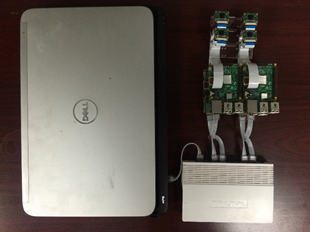
\includegraphics[height=5cm]{computer}}
  \subcaptionbox{拍摄时间检测系统}
      {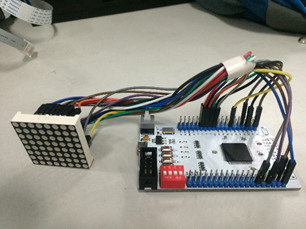
\includegraphics[height=5cm]{detect}}
  \caption{多摄像头系统及拍摄时间检测系统}
  \label{ss}
\end{figure}

\section{LED点阵编码方法比较}

本节主要对~\ref{codeMe}节所介绍的LED点阵编码方法进行实验对比。设置LED点阵的控制周期均为1ms,按照上文所介绍的方法分别进行编码。摄像头曝光时间为10ms,帧率为25fps,则相邻两帧图像之间的时间差理想情况下为40ms。

实验时,利用摄像头对LED点阵进行拍摄,获取连续的100帧图像,分析每帧图像内显示的点阵状态,计算相邻帧所拍摄到的点阵之间变化的时间间隔,与理论值40ms进行比较,从而确定各编码方法对拍摄时间的检测效果。实验结果如图~\ref{coding}所示,各编码方法检测结果的平均值和均方差如表~\ref{codingT}所示:

\begin{figure}[h] 
  \centering
  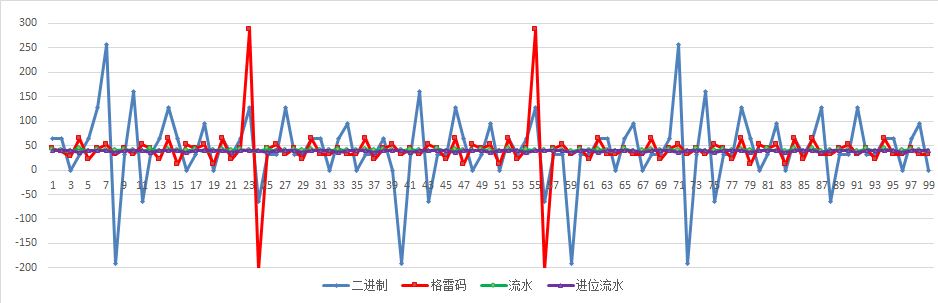
\includegraphics[height=5cm]{coding}
  \caption{LED点阵编码方法的拍摄时间检测结果比较}
    \label{coding}
\end{figure}

\begin{table}[h]
  \centering
  \caption{各编码方法检测结果的均方差值} 
  \label{codingT}
  \begin{tabular}{c|c|c|c|c}\hline
  &  二进制编码 &  格雷码编码 & 流水编码 &  进位流水编码 \\ \hline 
  平均值 & 41.37&39.86 &39.96&39.07\\ \hline
  均方差 & 74.45 & 51.74 & 1.82 &1.69\\ \hline
  \end{tabular}
\end{table}

通过实验结果可以看出,四种编码方法均可以检测到相邻帧之间的时间间隔,且检测的平值均在40ms左右。但采用二进制编码方法时,拍摄时间检测错误率较高,得到的两帧之间的时间差波动较大,计算得到的时间差均方差值也就较大,由于摄像机拍摄到的各帧图像中LED点阵发生叠加,导致检测到错误的相邻帧之间的时间间隔,最大错误值达到256ms。采用格雷码编码方法时,同样存在检测错误的情况,但检测错误率要优于二进制编码方法,检测结果均方差值也要优于二进制方法但仍有个别帧的检测误差较大,最大错误检测值为288ms。采用流水编码方法时,可以有效避免状态叠加造成的检测错误,使得检测结果的波动大幅减小,检测错误率远低于前两种方法,但由于该编码方法的总循环周期较短,在处理拍摄图像时,需要手动设置拍摄到的LED点阵所处的循环周期顺序,否则会对检测结果造成影响。采用进位流水编码方法时,能够得到最好的检测结果,检测误差最小且均方差值也最小,利用该方法能够实现对于摄像头拍摄时间的检测功能。

\section{摄像头拍摄时间检测}
\label{detSec}

本节主要介绍摄像头拍摄时间检测方法的实验验证。根据~\ref{detecSe}节所介绍的方法首先设置系统各项参数。为了提高检测精度,设置摄像头的曝光时间为2ms,帧率为25fps,设置LED点阵按照进位流水方法进行编码,每一行设置为一组,则整个LED点阵共分为8组。控制周期设置为50$\mu s$,则第一组每个LED灯的点亮的持续时间为50$\mu s$,第二组各个LED灯的点亮持续时间为$50 \times 8 = 400\mu s = 0.4ms$,则第二组所有LED灯依次发送亮灭变化,总的循环周期为$0.4 \times 8 = 3.2ms$。根据公式~\ref{5}可知,对于曝光时间长度为2ms的摄像头来说,其曝光时间长于第二组内单个LED灯点亮持续时间,短于第二组内所有LED灯总循环时间,因此其拍摄到的LED点阵图像当中,第一组内各个LED灯均点亮,第二组内部分点亮,第三至第八组内有一个或者两个LED灯点亮。在实际运行过程当中,拍摄到的一张LED点阵图像如图~\ref{2ms}所示,由于摄像头曝光时间较短,可以看到图像亮度较低,但是LED灯较为明亮,能够正确进行识别。然后根据~\ref{detecSe}节所介绍的方法,对拍摄到的图像进行识别,计算摄像头的真实拍摄时间,计算结果如图~\ref{2msR}所示。

\begin{figure}[h] 
  \centering%
    \subcaptionbox{摄像头拍摄到的LED点阵图像\label{2ms}}
    {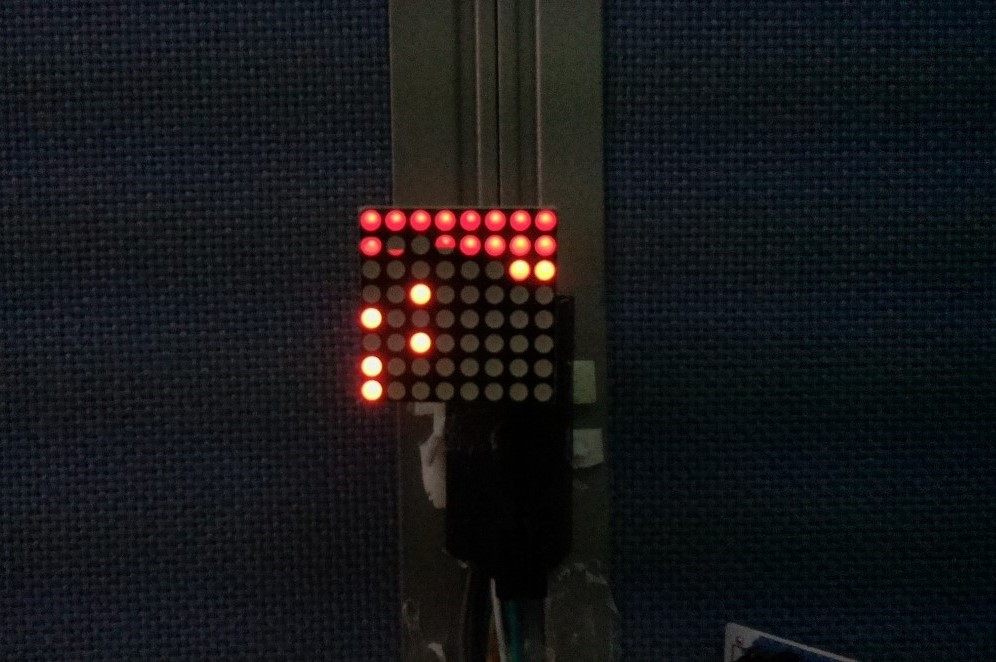
\includegraphics[height=4.5cm]{2ms}}
  \subcaptionbox{拍摄时间计算结果\label{2msR}}
      {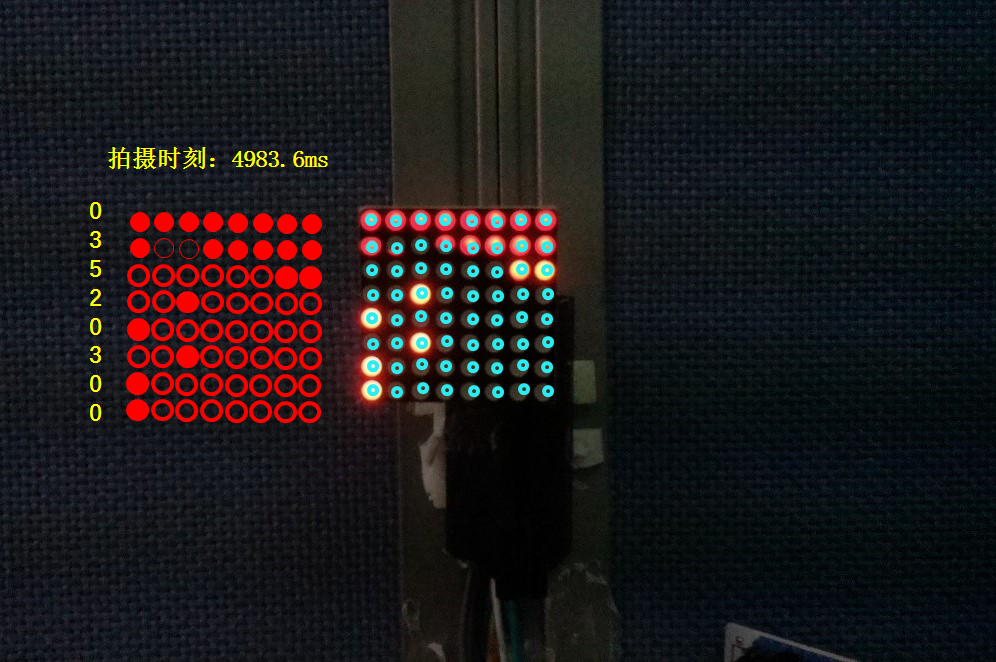
\includegraphics[height=4.5cm]{2msR}}
  \caption{摄像头拍摄时间检测}
\end{figure}

为了验证检测结果的正确性,连续拍摄100张LED点阵图片,每两帧之间设置一定的时间间隔。读取摄像头给每帧图像设定的拍摄时间戳,计算两帧图像之间的时间间隔。同时根据拍摄时间检测算法根据LED点阵状态检测拍摄时间,计算两帧图像之间的时间间隔。摄像头设定的时间戳由Linux操作系统计算,精度能够达到微秒级别,通过LED点阵计算的拍摄时间根据上文所介绍的参数设置,可达到$400\mu s$。计算结果如图~\ref{stamp}所示,平均值和均方差如表~\ref{codingT}所示:

\begin{figure}[h] 
  \centering
  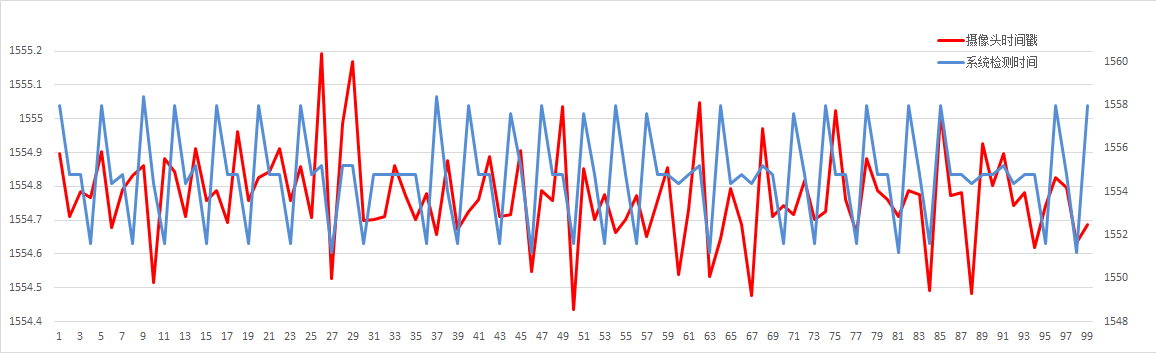
\includegraphics[height=5cm]{stamp}
  \caption{系统检测时间与摄像头时间戳时间比较}
    \label{stamp}
\end{figure}

\begin{table}[h]
  \centering
  \caption{各编码方法检测结果的均方差值} 
  \label{codingT}
  \begin{tabular}{|c|c|c|}\hline
  &  平均值 &  均方差 \\ \hline 
  时间戳 & 1554.7703 &0.1367\\ \hline
  LED点阵检测 & 1554.7313 & 2.1968\\ \hline
  \end{tabular}
\end{table}

由计算结果可以看出,本文提出的拍摄时间检测方法与利用时间戳计算出的结果基本一致,每两帧图像之间的时间差的计算平均值仅相差$40\mu s$左右。但是受该检测方法的精度限制,其检测结果的相对于利用时间戳计算的结果波动较大,均方差值略大,但仍处于合理波动范围内,利用该方法能够准确有效地检测摄像头的拍摄时间。

\section{多摄像头系统时间同步}

本节利用上文所述的多摄像头系统对时间同步方法进行验证。系统中共包含4个树莓派电脑,每个电脑连接一个摄像头进行拍摄,树莓派与图像处理服务器通过交换机连接,处于同一个局域网内,可以进行信号交互和数据传输。摄像头和LED点阵的参数设置与~\ref{detSec}节所介绍的参数相同。

在系统正常运行的过程中,当需要对拍摄时间进行检测时,将检测LED点阵置于各个摄像头的视野当中,利用服务器控制各个摄像头同时保存一帧LED点阵图像,并回传给服务器,服务器根据图像中LED点阵状态计算各个摄像头的拍摄时间差,处理结果如图~\ref{4unsync}所示。

\begin{figure}[h] 
  \centering%
  \subcaptionbox{同步前拍摄结果 \\ .\label{4unsync}}
    {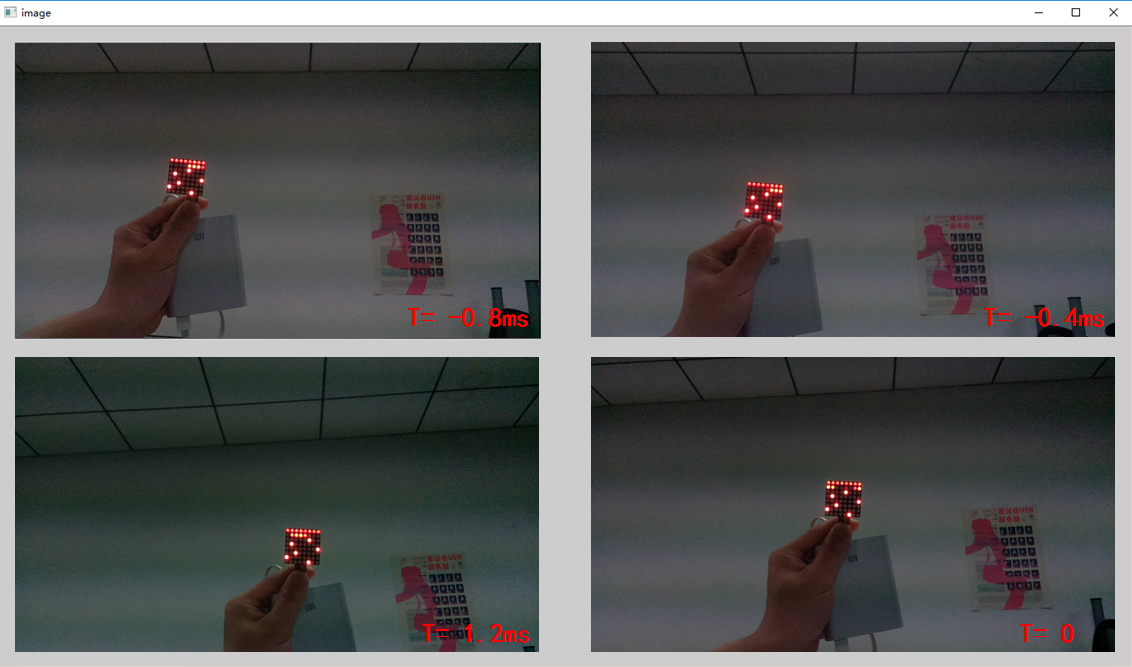
\includegraphics[height=9cm]{4unsync}}
    \subcaptionbox{同步后拍摄结果\label{4sync}}
    {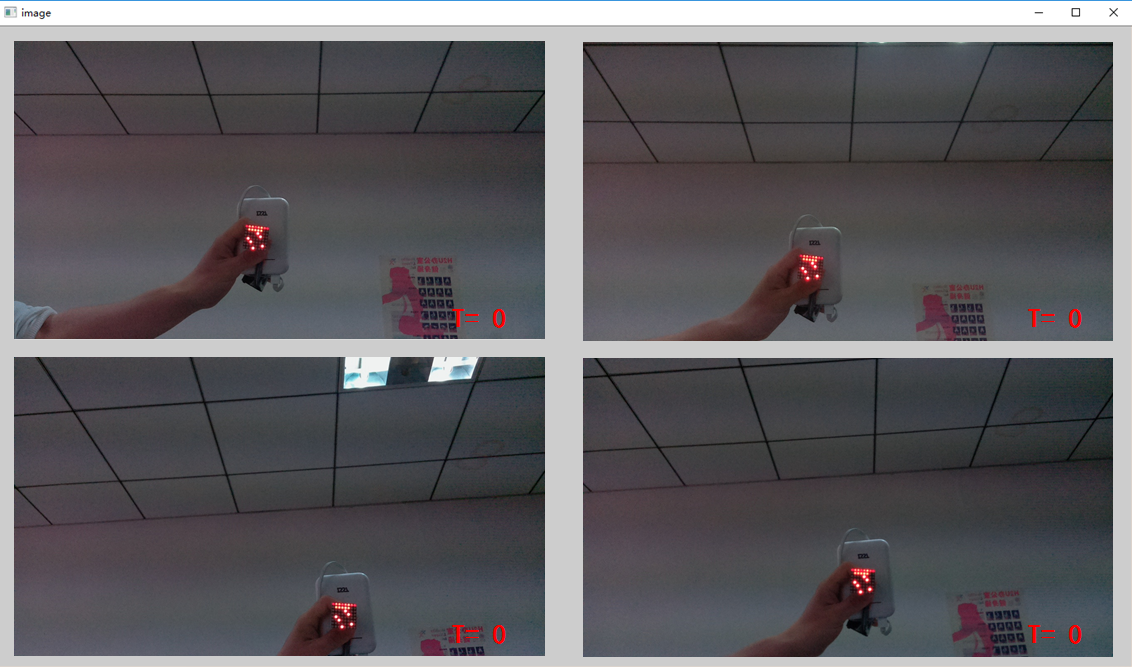
\includegraphics[height=9cm]{4sync}}
  \caption{多摄像头系统拍摄结果}
\end{figure}

从图中可以看出,系统内各个摄像头的拍摄角度不同,但都能够保证LED点阵处于视野范围内。保存的图像中,LED点阵的状态不同,说明虽然服务器控制摄像头在“同一”时刻保存图像,但由于各个摄像头的拍摄时间存在差异,实际拍摄到的图像因此不同。当服务器获得LED点阵图像后,对图像进行处理,检测各个摄像头的拍摄拍摄时间。如图可知,4号摄像头的拍摄时间处于中间位置,选取其作为基准摄像头,计算其他摄像头与其的拍摄时间差。然后根据~\ref{proSec}节所介绍的方法计算各个摄像头需要暂停的时间长度,由服务器向各个摄像头分别发送控制信号,调整其拍摄时间。调整后的最终的同步结果如图~\ref{4sync}所示。

\section{本章小结}

在本章中,通过树莓派电脑和图像处理服务器构建了一个多摄像头系统。该系统利用树莓派控制摄像头,通过局域网络与服务器连接,由服务器处理各个摄像头拍摄到的图像数据,并控制摄像头调整同步。该系统具有一定的可扩展性,能组成大规模的多摄像头系统。利用该系统分别对几种LED点阵编码方法进行了比较,验证了进位流水编码方法具有更高的检测精度和更好的叠加可识别性。本章还对摄像头拍摄时间的检测方法和多摄像头系统的同步方法进行了实验验证,通过实验可以看出两种方法都具有较高的实验精度,能够实现设计功能。



























































